%%
%% This is file `example/ch_intro.tex',
%% generated with the docstrip utility.
%%
%% The original source files were:
%%
%% install/buptgraduatethesis.dtx  (with options: `ch-intro')
%% 
%% This file is a part of the example of BUPTGraduateThesis.
%% 

\chapter{绪论}
\section{研究背景及意义}
随着互联网的发展,云数据中心的规模不断扩大,业务流量不断变化,如何为租户提供可编程的云数据中心网络,如何对云数据中心的流量进行有效的控制,提高带宽的利用率,降低成本,成为目前急需解决的问题。

\gls*{SDN}作为一种新兴的可编程网络架构,有动态配置、可编程及快速响应的特点。其核心思想是将网络控制平面与数据转发平面分离,实现控制平面对数据平面的全局集中化控制;同时对外提供开放的可编程接口,为网络提供可编程能力。控制权的迁移使得底层构架能够抽象出来,各种应用和网络服务因此能将网络当作一个逻辑或虚拟实体,不再依赖于底层网络设备\cite{SDN-1},使得网络配置的自动化程度得到极大提高。通过应用\gls*{SDN},除了网络的设计和操作变得简化,网络设备也得到简化,这些设备无需理解或处理成千上万的协议,只需要接受\gls*{SDN}控制器的指令即可。利用集中控制,网络管理员可以实时改变网络的行为,并且在几小时或几天内就可以部署新的应用和网络服务。

网络虚拟化\cite{Virtual-1}是一种将底层网络中的硬件以及配套的软件资源进行整合,形成统一管理实体的技术,通过虚拟网络资源到物理网络资源的映射,使得多个逻辑虚拟网络共享底层物理网络基础设施,为用户提供差异化服务。网络虚拟化技术是当今网络革新的重要技术之一。从概念上,网络虚拟化与\gls*{SDN}是互相独立的,但随着近几年网络技术的发展与融合,二者之间的联系变得越来越紧密,\gls*{SDN}的技术相关专题常会提及网络虚拟化技术,网络虚拟化问题的研究也时常会运用到\gls*{SDN}的概念,可见基于\gls*{SDN}的网络虚拟化技术已经成为网络技术研究领域的一个专门课题。

OpenStack\cite{Openstack-1}是由Rackspace和美国国家航空航天局(NASA)合作研发的用于搭建Iaas平台的云计算管理软件。旨在为公共及私有云的建设与管理提供软件的开源项目,主要提供计算、存储、网络服务。OpenStack支持几乎所有类型的云环境,项目目标是提供实施简单、可大规模扩展、丰富、标准统一的云计算管理平台。OpenStack通过各种互补的服务提供了基础设施即服务(IaaS)的解决方案,每个服务提供API以进行集成\cite{Openstack-2}。

在现有OpenStack云平台中,租户网络的创建与隔离仅限于服务器内部,OpenStack无法进行物理服务器之间数据中心网络的管控,跨服务器的通信通过隧道技术实现,该模式无法满足用户多样性的需求,同时无法实现云数据中心带宽资源的有效利用,时常会出现有些链路阻塞严重,而有些链路则处于空闲状态。

本文以此作为出发点,提出了一种多租户虚拟网络定制化管理方案,运用虚拟化技术,为租户提供相互隔离的\gls*{vSDN},完成云数据中心物理资源有效利用的同时,\gls*{SDN}网络由租户自有的控制器实现集中管控,租户可以实时监测当前的流量状况并根据流量状况自定义转发路径,实现对网络的灵活管控,在不降低云平台性能的前提下,实现了OpenStack云平台中租户网络的定制化操作,既提高了安全性,又可以根据当下链路的剩余带宽,进行链路的定制化,提高带宽的利用率。对于租户本身而言,真正实现了租户对全局网络的可控性。对于运营商来说,对物理网络的集中控制可以大大较小网络配置的繁琐性,可以对网络故障实现快速的排查,提高可扩展性。

\section{主要研究内容及创新点}
\subsection{研究内容}
本课题为实现基于\gls*{SDN}的云平台多租户虚拟网络定制化方案,将\gls*{SDN}集成到云数据中心,通过虚拟化技术,为租户提供了可编程的\gls*{vSDN}网络,\gls*{vSDN}网络由租户自由的\gls*{SDN}控制器进行集中管控,租户可以根据当前的链路状况,进行定制化流表的下发,真正实现对网络的灵活定制化操作。主要包括以下三个方面的研究内容:

第一、实现虚拟网络的创建:通过虚拟化技术,实现跨物理服务器,数据中心网络的虚拟化,虚拟网络支持SDN模式,由租户自己的SDN控制器实现集中管控,本文选用\gls*{OVX}\cite{OVX-1}实现虚拟网络的创建。对于底层物理设备来说,OVX是一个控制器;对于租户控制器来说,OVX可以看做是OpenFlow交换机的集合,租户控制器看到的只是一张虚拟网络。OVX最大的优势是紧密结合了SDN,可以发挥SDN的控制与转发分离的强大优势,将创建的虚拟网络指定SDN控制器,从而可以运用SDN的优势,实现对租户虚拟网络的管控。

第二、完成虚拟网络的集中控制:

第三、云平台前端可视化操作:

\subsection{创新点}
针对现有云平台数据中心的不足,本文主要实现了SDN与云平台的结合,将SDN的集中控制、网络的虚拟化集成到云平台中,实现了租户网络隔离的同时,租户可以对网络实现自由控制。相应的创新点主要涉及以下几个方面:

\begin{enumerate}
\item 对于云平台运营商来说,物理网络的集中控制,可以有效的减小网络配置的繁琐性,为数据中心规模的伸缩性提供了便利,对网络的状况可以实现实时监控,同时大大加速了网络的故障修复速度,通过控制侧的日志输出,以及错误模拟,实现快速故障排除。
\item 将虚拟化技术集成到云数据中心,为租户提供相互隔离的\gls*{vSDN}网络,该网络由租户自己的控制器实现集中控制。集中控制的实现,可以让租户指定灵活的数据包转发路径,以及灵活的转发策略。对于自身网络的变化也可以实现即时的应对措施。从而对现有的网络资源进行最有效的利用,减少了网络资源的浪费。租户之间的隔离性,保证了租户数据传输的安全性。
\item 基于包对技术,完成了虚拟网络的链路带宽测量,实现了细粒度的剩余带宽测量,精确度远远高于以前的模式;基于数据包统计的方法,实现了粗粒度的已用带宽的测量;完成了\gls*{SDN}架构下的时延测量。租户根据带宽、时延实现定制化链路的选取,可以有效的利用剩余带宽,将降低数据传输时延,大大加快了数据中心网络的传输速度。
\end{enumerate}

综上所述,基于\gls*{SDN}的云平台多租户虚拟网络定制化方案,对提高云数据中心的带宽利用率,为租户提供可编程的云网络是非常必要的,有助于实现租户网络的定制化操作,同时为运营商进行云数据中心的维护和配置提供了便利。

\section{研究生期间主要工作}
\section{论文组织结构}


\begin{enumerate}
\item 第二章介绍……
\item ……
\end{enumerate}
\begin{itemize}
\item 第二章介绍……
\item ……
\end{itemize}
图\ref{fig:env1}
\begin{figure}[!htb]
  \centering
  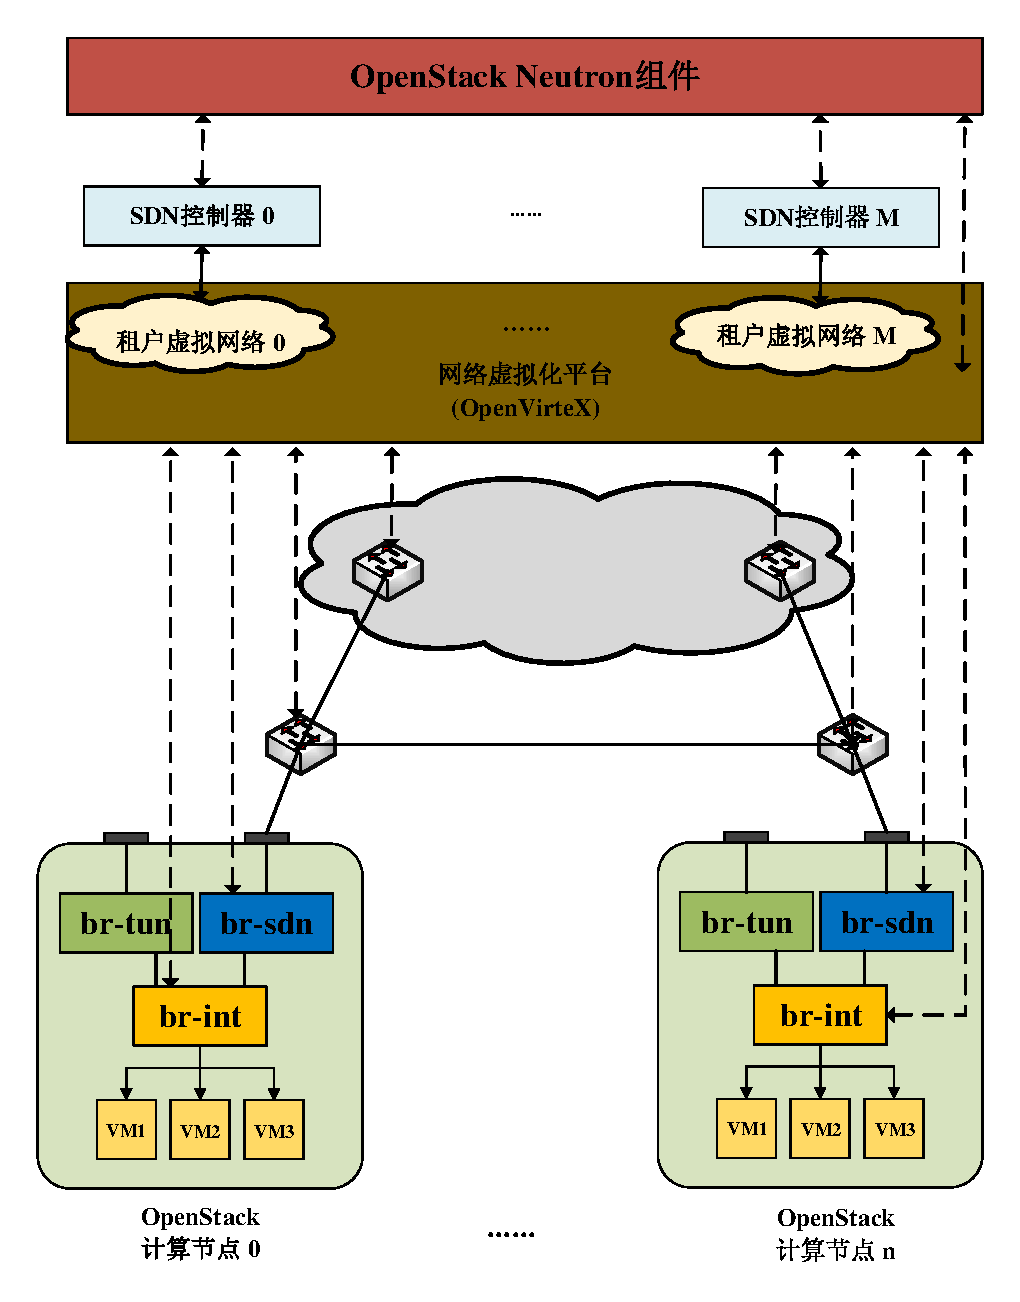
\includegraphics[width=100mm]{logo/architecture}
  \caption{System environment.}
  \label{fig:env1}
\end{figure}

%% 本章参考文献
\ifx\usechapbib\empty
\nocite{BSTcontrol}
\setcounter{NAT@ctr}{0}
\bibliographystyle{buptgraduatethesis}
\bibliography{bare_thesis}
\fi
